\documentclass[a4paper]{article}
\usepackage{apacite}
\usepackage{pdfpages}
\usepackage{titling}

\setlength{\droptitle}{0em}   % This is your set screw

\usepackage{datatool}% http://ctan.org/pkg/datatool
\newcommand{\sortitem}[1]{%
  \DTLnewrow{list}% Create a new entry
  \DTLnewdbentry{list}{description}{#1}% Add entry as description
}
\newenvironment{sortedlist}{%
  \DTLifdbexists{list}{\DTLcleardb{list}}{\DTLnewdb{list}}% Create new/discard old list
}{%
  \DTLsort{description}{list}% Sort list
  \begin{itemize}%
    \DTLforeach*{list}{\theDesc=description}{%
      \item \theDesc}% Print each item
  \end{itemize}%
}

\bibliographystyle{apacite}

\title{Project-oriented Course with Triband: \\
  \large A Reflection Report}
\author{Jonas Haugesen}
\date{December 2017}

\begin{document}

\maketitle

\tableofcontents

\section{Introduction}


\section{Formalities}
The internship were in collaboration with the small game studio, Triband. The internship ran from September to December 2017 and working hours were 20 per week. During the time of the internship Triband were developing two games and two prototypes. The two games were Keyboard Sports and Golf All the Things and the two prototypes were Madkamp and Torstens Mund. I was working on all of these except Keyboard Sports. None of the games or prototype have been released to the public. My role during the internship was Game Designer and in practice I worked on game mechanics, art, implementation, programming and level design. My contribution in the different projects has been considered valuable and will as of writing be apparent in any final release.


\section{Projects}
During my internship I worked on two prototypes and one game. The two prototypes were made in accordance to a partnership between Triband and Made in Copenhagen and were made to support a cartoon series for the Danish television network Danmarks Radio. The game is a game for mobile devices that is currently in development and planned for release in the first half of 2018 and with a consecutive PC release. The two next sections will cover the two projects and after this a summary will be given.


\subsection{Torsten Spis P{{\ae}}nt}
Torsten Spis P{\ae}nt is an original cartoon series in active development. It is about a young boy who is living with his mom in {\O}restaden, Copenhagen and his exploration of new and exciting food. In the pilot episode, Torsten's mom cites the old phrase "you are what you eat," and the gullible Torsten takes this as fact, letting his imagination bring him into the world of animated fruits and vegetables. \newline
As part of the publishing deal for Torsten Spis P{\ae}nt a series of accompanying games is required. The series is in early development and has yet to be greenlit. For this to happen, content needs to be presented and accepted. Part of this content is prototypes for future games, and that is where Triband enters the partnership. Triband made a series of very rough prototypes to explore different game mechanics. The best two were selected and the actual development of two prototypes were tasked to me and the other intern at Triband. The work was divided with the other intern producing the art and animation, and me the programming and implementation. The mechanics of the two prototypes were previously decided on so the amount of design work were limited.

\subsubsection{Madkamp}
Madkamp, or \textit{Food Fight}, is a game concept where the player is brought into Torsten's kitchen to, as the title suggest, fight with food. The player can look around the kitchen by utilising the mobile device's gyroscope and touch the screen to throw a random fruit or vegetable. \newline
Before starting the process we received some instructions on what the prototype had to contain:
\begin{itemize}
  \item Start screen including:
  \begin{itemize}
    \item Big play button
    \item Instructions button: Hit Torsten with the food. Raise the phone and look around to aim
  \end{itemize}
  \item End screen (appears after $\approx$45 seconds) including:
  \begin{itemize}
    \item Score: How many times you hit Torsten
    \item Play again button
  \end{itemize}
\end{itemize}
Additionally, a small model of the kitchen was made beforehand to better visualise the possibilities of the room (see figure \ref{kitchenmodel}).
\begin{center}
  \begin{figure}[!htb]
    \noindent\makebox[\textwidth]{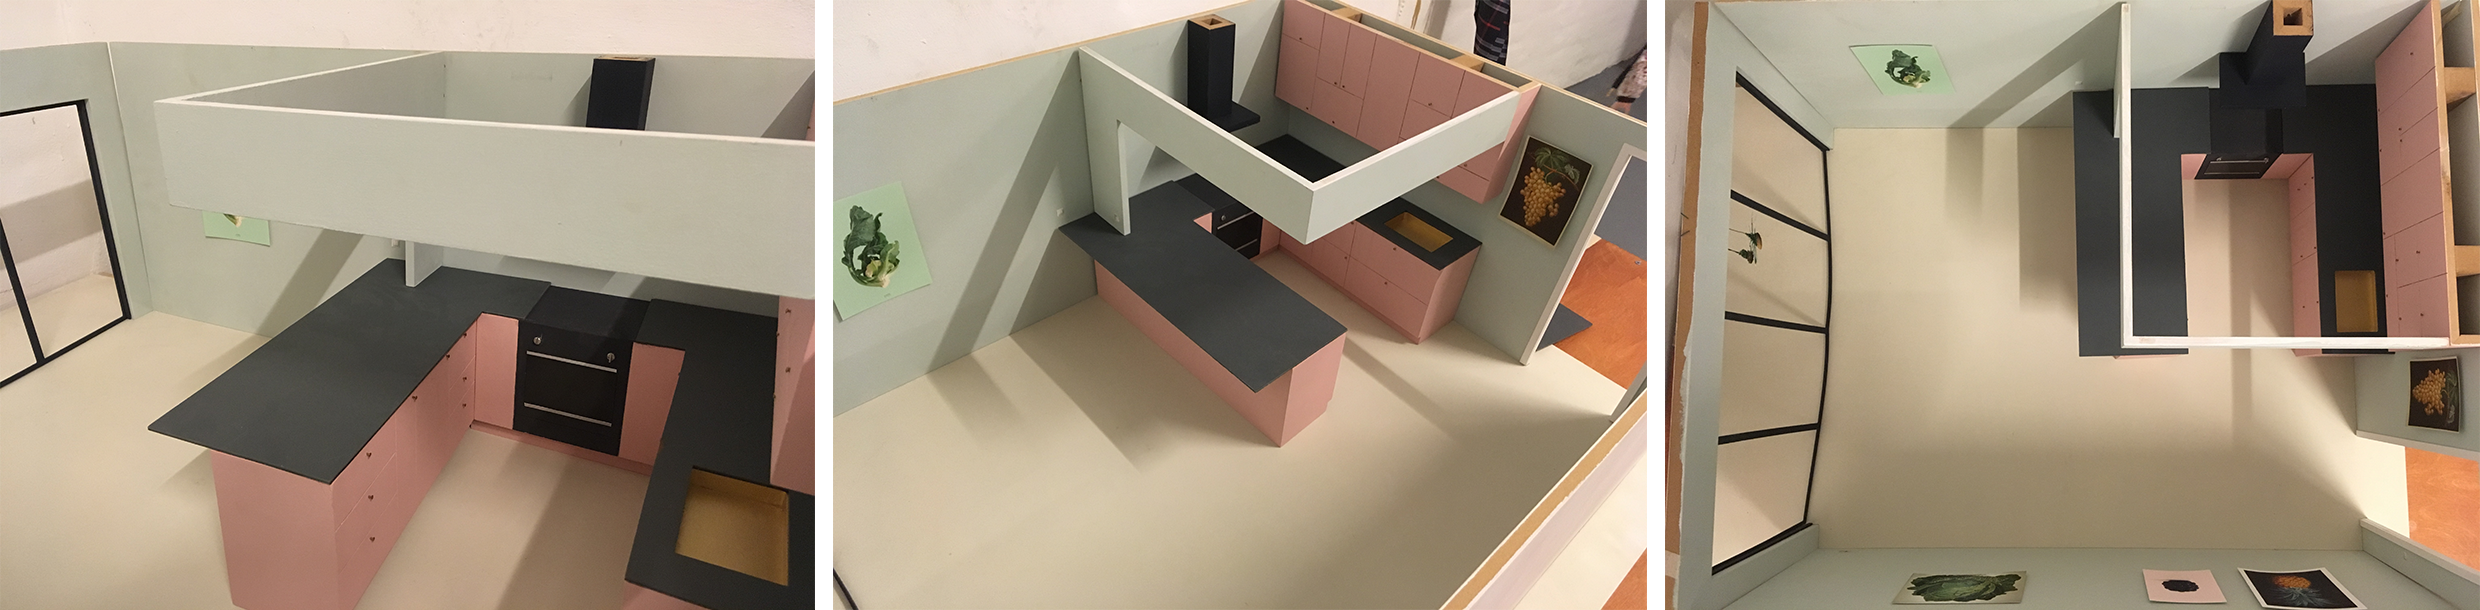
\includegraphics[width = \paperwidth]{Madkamp/KitchenModel}}
    \caption{A Model of Torsten's Kitchen}
    \label{kitchenmodel}
  \end{figure}
\end{center}
The work was then initiated with a division of labour. Art would be made by the other intern and implementation of controls and mechanics to me. I quickly set up a test level with some target practices to prototype the gyroscope and throwing controls (see figure \ref{TestScene}A). The gyroscopic input proved no difficulty but as I implemented the throwing mechanic I quickly realised that, to not confuse the player, the origin of all projectile needed to be centred on the screen and be projected in the orientation of the view. Originally, I wanted the player to be able to shoot from anywhere on the screen and shoot in the direction of the point in the game world the input was pointed at. Very quickly, however, this was deemed to be too complex for the target audience, so I chose to simplify the mechanic to the previously described mechanic.

Next challenge was visualising the point of impact for the projectiles in the form of splats. My first attempt at this was to simply spawn a sprite at the point of collision and rotate it according to the normal of the surface. For this to work the size of the sprite would have be adjusted according to the proximity of the closest edge of the surface. I accomplished this by stepping in four opposite directions iteratively and the first step that was not on the collision's surface determined the size of the sprite according to the distance between the collision point and the closest edge (see figure \ref{TestScene}B). The problem of this approach at visualising splats is that splats close to an edge will be miniscule, where a similar splat in the real world would instead wrap around the edge and continue on the next surface. Thinking that these splats were at the centre of what would make this game amusing, I scrapped this approach because I decided that it had no possibility of resulting in a satisfactory result. Instead I focused on an approach that utilised UV mapping \cite{mullen}. In brief, the 3D model that is capable of being hit by the projectiles has two UV maps: 1) On the top, a regular texture map. 2) On the bottom, a texture map with all surfaces covered in the splat material. Each time the model is hit, the surrounding area exposes the bottom layer with the splat material (see figure \ref{UVSplat}).
\begin{center}
  \begin{figure}[!htb]
    \noindent\makebox[\textwidth]{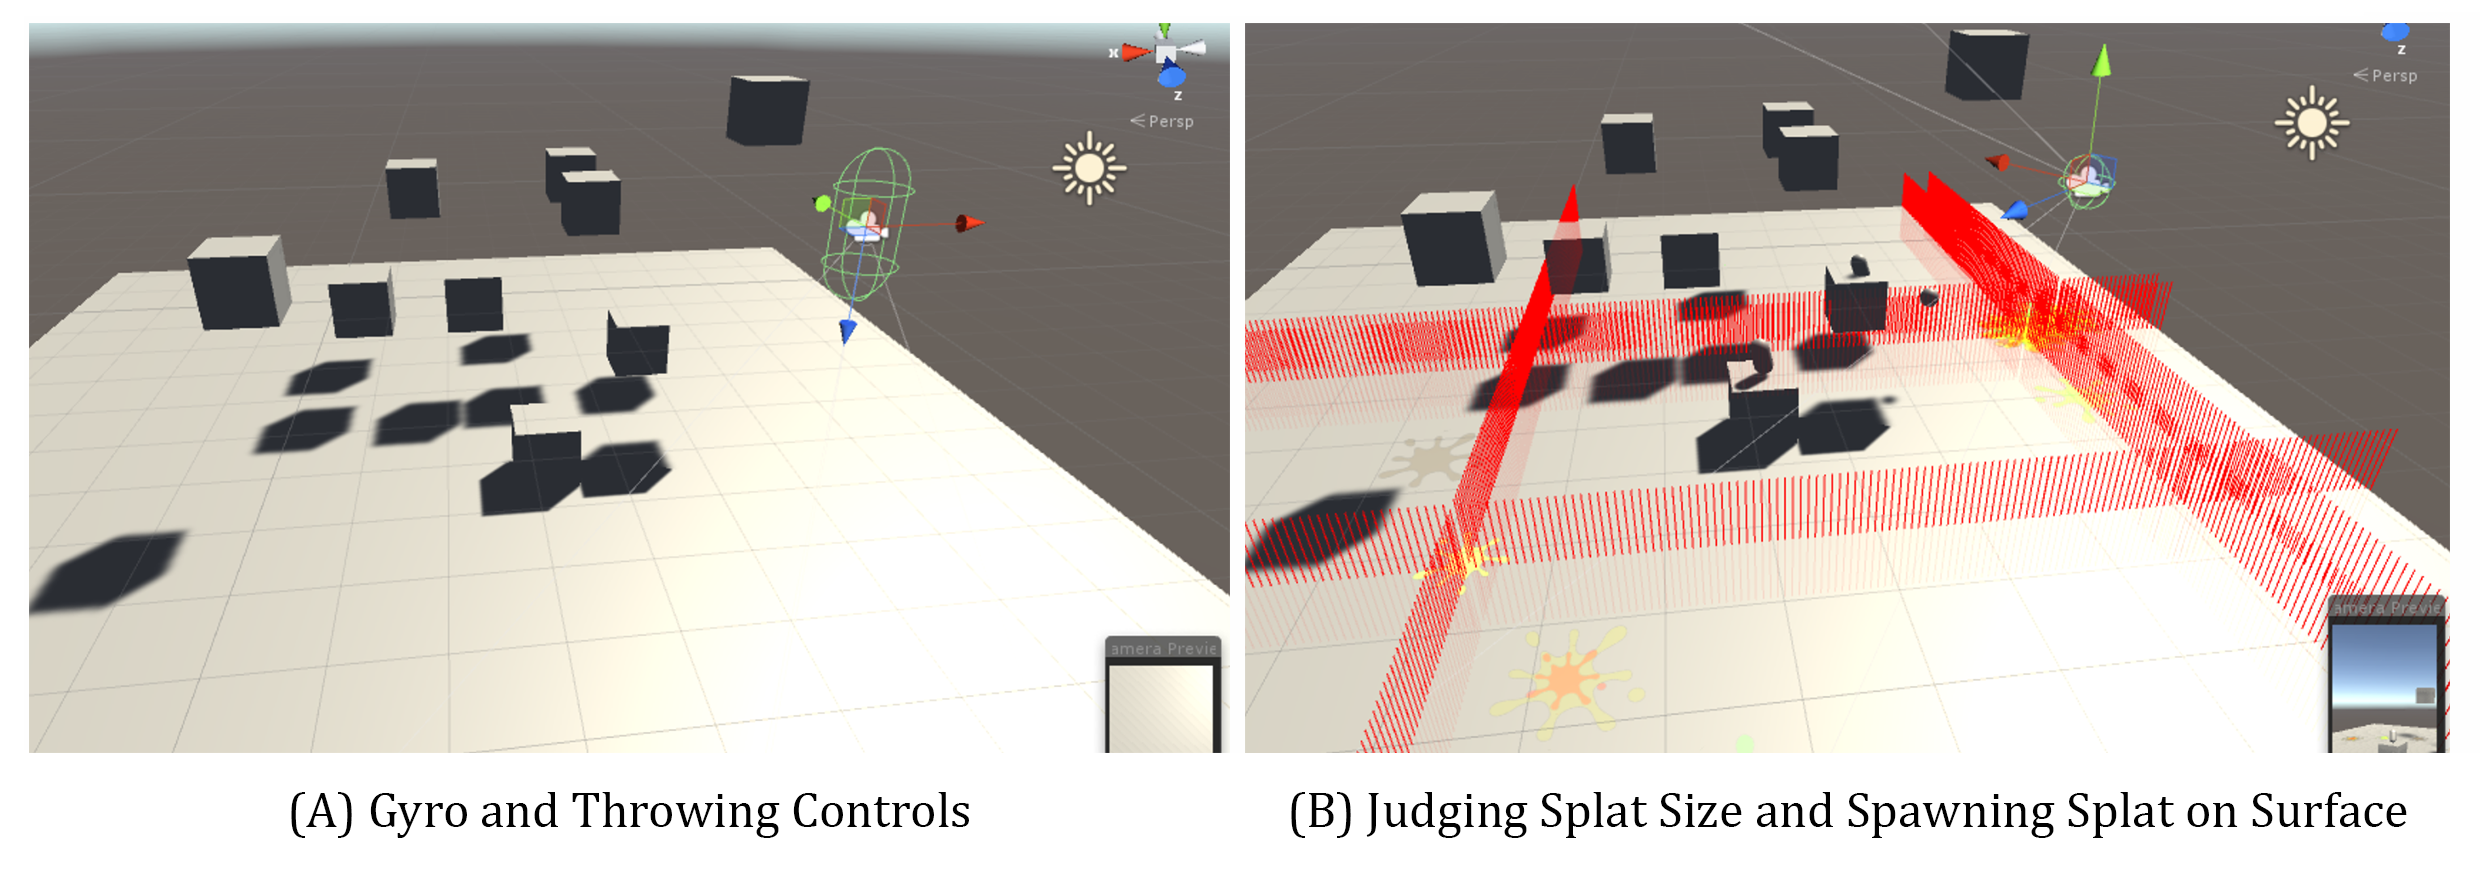
\includegraphics[width = \paperwidth]{Madkamp/TestScene}}
    \caption{The Test Level}
    \label{TestScene}
  \end{figure}
\end{center}
\begin{center}
  \begin{figure}[!htb]
    \noindent\makebox[\textwidth]{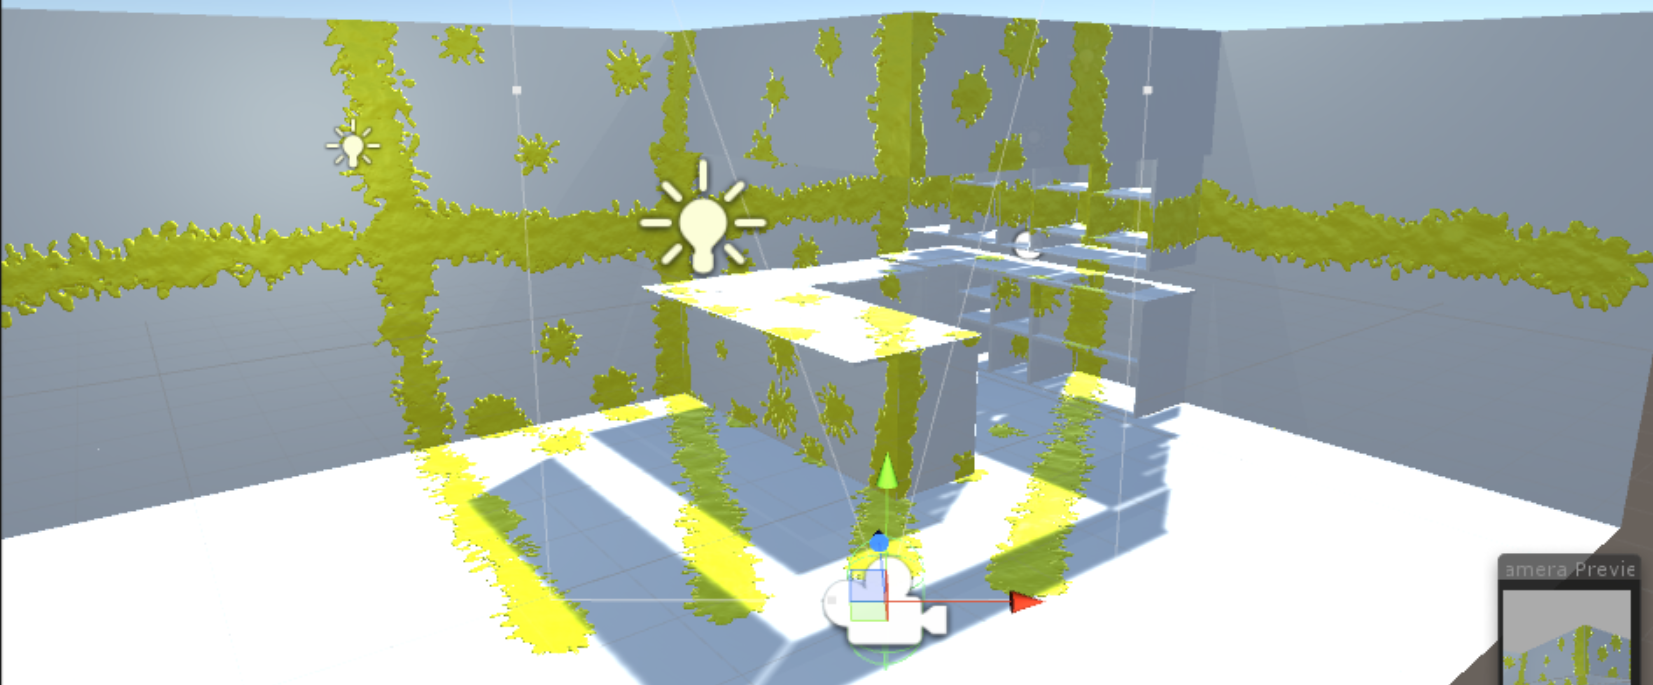
\includegraphics[width = \paperwidth]{Madkamp/UVSplat}}
    \caption{UV Mapping Splat Approach}
    \label{UVSplat}
  \end{figure}
\end{center}
The rest of the prototype was fairly simple. In the final level a placeholder for Torsten is set on a track around the kitchen and as soon the line of sight between Torsten and the player is unobstructed, Torsten will throw projectiles at the player in a predefined rhythm. To dodge Torsten's projectiles the player can look away from the approaching fruit or vegetable.
\subsubsection{Torstens Mund}
Torstens Mund, or \textit{Torsten's Mouth}, is a concept for a playful application. It is a playful application instead of a game because it does not contain any type of conflict and there is no quantifiable outcome of the play activity \cite[ch. 7, p. 11]{salen}. In Torstens Mund, the player is situated inside of Torsten's mouth and is able to look out through his open mouth. It is developed for mobile devices and utilises the built-in camera in such devices, so the world portrayed outside of the mouth is the real world as seen through the camera. When the player touches the device's screen Torsten starts chewing, on a still image of what was visible at the time of the input, and gives his impression of what that tastes like.

We initiated the work with a division of labour: The other intern would do art and animation and I would implement controls and mechanics. The first problem was how to integrate the camera feed into the prototype. This proved to be difficult mainly because it involved getting permissions, screen orientation and resolution from the device and obsolete documentation. Once I had the camera feed I needed to visualise it somehow. I did this by assigning it to the texture of an in-game object. The next challenge was to capture a still image and have the mouth chew on it. I figured that the simplest, possibly not best, solution, was to animate a simple rectangle to simulate the crumbling of something being chewed (see figure \ref{ChewAni}).
\begin{center}
  \begin{figure}[!htb]
    \noindent\makebox[\textwidth]{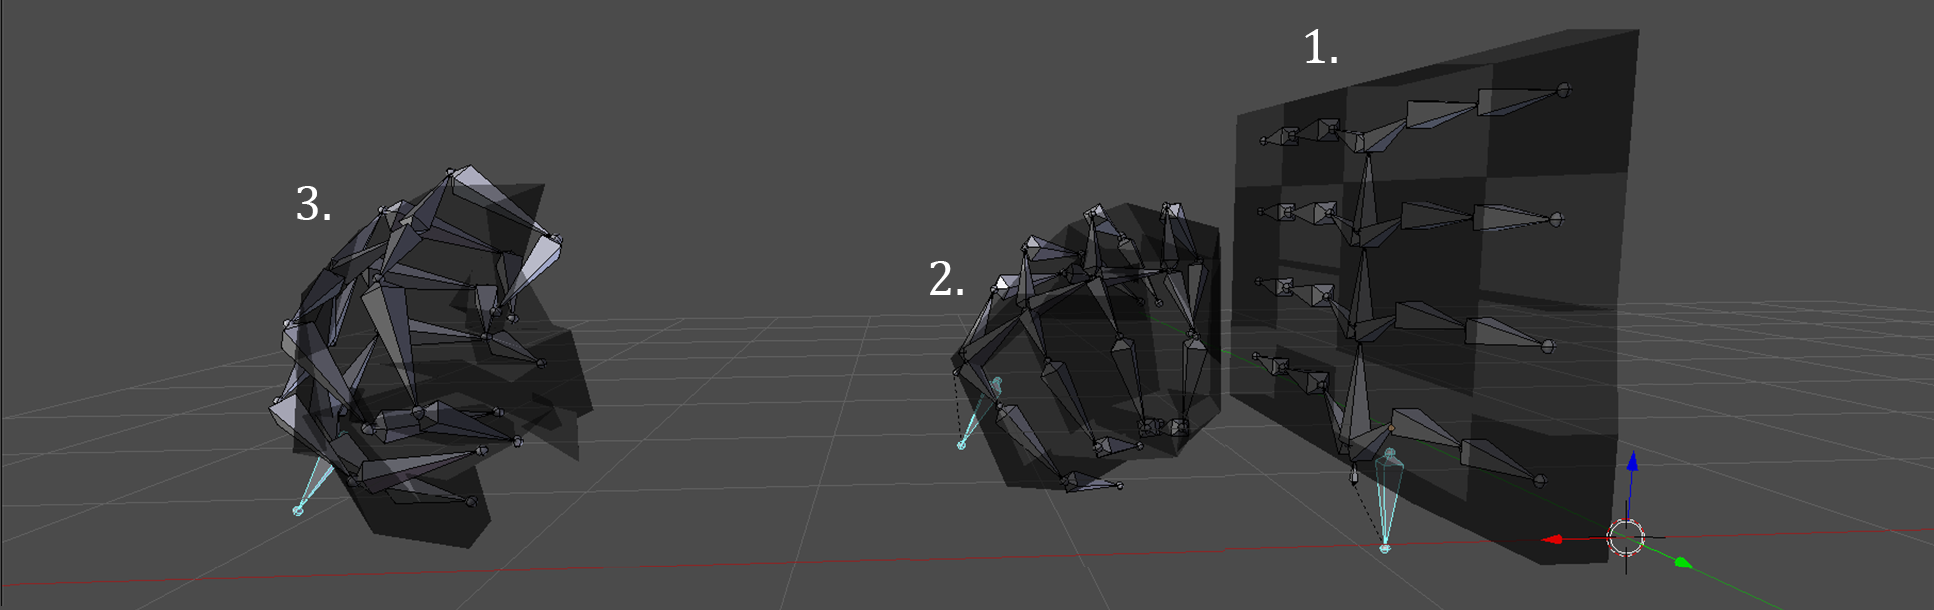
\includegraphics[width = \paperwidth]{TorstensMund/ChewAnimation}}
    \caption{The Animation Timeline of the Still Image being Chewed}
    \label{ChewAni}
  \end{figure}
\end{center}
The impression Torsten expresses after having chewed on something is based on the average colour of a square section of the centre of the still image. A random sound clip corresponding to the colour is then played. Examples of these follows:
\begin{itemize}
  \item Yellow: Ew, this tastes like pee.
  \item Blue: This tastes like jellyfish, or something like that.
  \item Brown: Pew, this tastes like sour underpants.
  \item Green: I like this, this tastes like a cucumber.
\end{itemize}


\subsection{Golf All the Things}
Golf All the Things is a game currently under development. When my internship started a number of levels had already been made and were being tested. The first levels are similar to an ordinary golf game, but gradually more and more wacky elements are incorporated. In one level, instead of shooting the golf ball across the field, the player propels the golf player himself towards the hole. In another level, the player plays as an elephant being kidnapped by some evil-doers. The general mechanic is that the player touches a point on the screen, moves the finger in a desired direction and lifts the finger. The line between the initial point and the point of release defines the amount of force and direction is applied in the game.

I was tasked with coming up with similar levels to the ones described above, or building previously pitched level ideas. The existing ideas were managed on a central bulletin board and organised according to the development process (see figure \ref{Bulletin}). Here, creativity was welcome and I managed my own levels completely. This allowed me to use my design knowledge and challenged my programming skills, since I would have to create the levels entirely on my own. Another interesting challenge was to get an overview of a project that had been in development for a duration. It really promoted the essentiality of structure in naming and folder conventions.
\begin{center}
  \begin{figure}[!htb]
    \noindent\makebox[\textwidth]{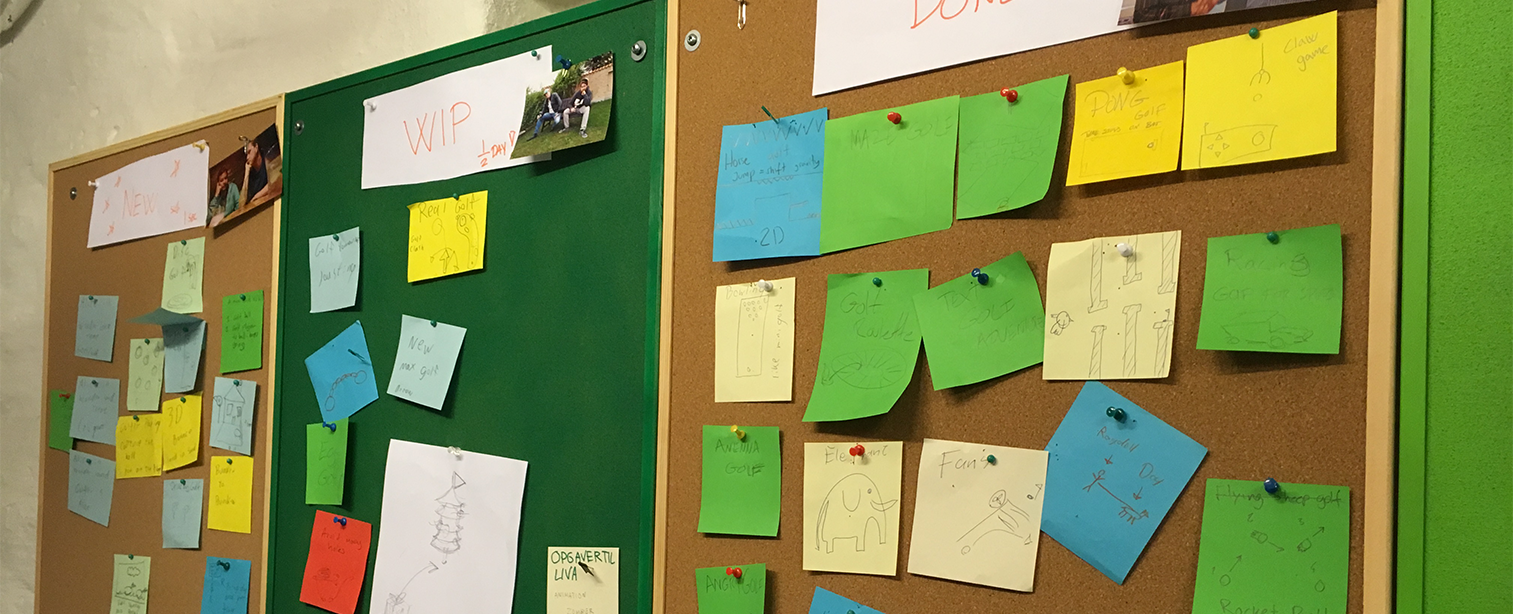
\includegraphics[width = \paperwidth]{Golf/Opslagstavle}}
    \caption{Bulletin Board for Golf Levels Ordered by New Ideas, Work in Progress and Done}
    \label{Bulletin}
  \end{figure}
\end{center}
\subsubsection{Paper Plane Golf}
My first idea for a level was one where the golf ball is a paper plane. You act on the plane by blowing wind behind it. The direction you shoot and the amount you pull back, determines the wind direction and the blow force of the wind. The challenge is to go through some hoops as you make it to the flag at the end of the level. If you fall too far down the player gets reset and if the player blows in a direction too disparate from the direction the plane is heading, the blow force is lessened, simulating a similar situation in the real world.

Being the first level most of the challenges were getting an overview of how the pre-existing assets could aid me in the creation. As examples: The ground shape creation tool, the golf shooter and controller base class, The triggers used for triggering an out-of-bounds-event and the tags used for identifying elements such as golf balls and golf goals. As I have experienced in other projects, disarray has a way of sneaking into planned structures, and this was true also for this project but in a much more limited way than I had previously experienced. Even this small amount of disorder, however, spurred a tidying some time midway in my internship, further instilling a respect for order in me.

Another challenge that arose from the paper plane level, was the fact that a locked outlook behind a propelled object, does not allow for much relative perspective: As the paper plane approached the hoops I had positioned in the sky, it proved hard to judge the relative distance between the paper plane and the hoop, resulting in premature or late actions. Pitching the view forward solved this challenge slightly, but made planning ahead more difficult, since an approaching hoop was only apparent as the paper plane neared it. Since, however, any polish of levels were not part of the current development cycle, this status was deemed good enough, and I moved on with a new level.
\begin{center}
  \begin{figure}[!htb]
    \noindent\makebox[\textwidth]{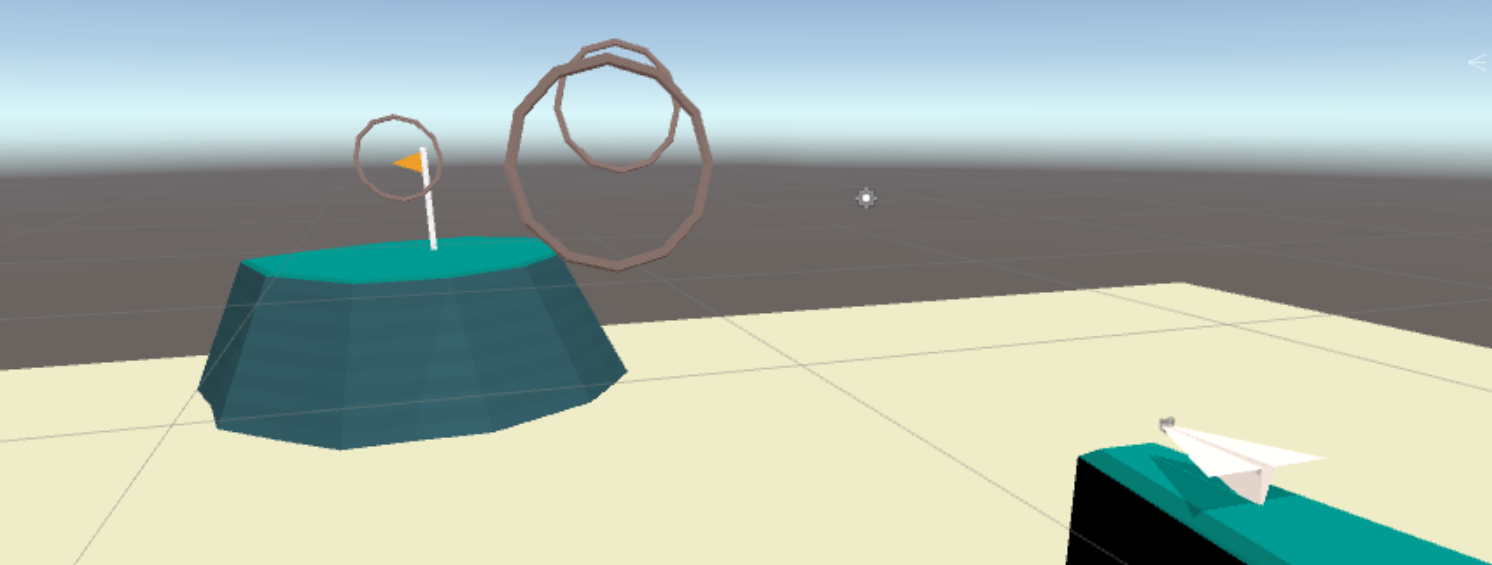
\includegraphics[width = \paperwidth]{Golf/PaperPlane}}
    \caption{The Paper Plane Level}
    \label{PaperPlane}
  \end{figure}
\end{center}
\subsubsection{Fishing Golf}
Next, was Fishing Golf. Here, the golf game was meant to be put in the context of a fishing trip. The first idea was a level in a first-person perspective and using the mobile device's gyroscope to look around. The goal was for the player to shoot out his/her fishing floater into the area where the water signalled the presence of fish. When the fish had latched on to the hook, the player should reel in the fish - level complete. This level proved to mainly be challenging in the creation of \textit{signifiers} \cite{norman}. Generally, there were three challenges in regards to signifiers: 1) Signalling the presence of fish in a certain area of the water. 2) Indicating that a fish had latched onto the hook. 3) Illustrating that having reeled in the fish completes the level. The first challenge was tackled by giving the visual cue of small waves, the second challenge I dealt with by using the vibration functionality of the mobile device, and the third challenge, the other intern and me tackled by modelling a fish that resembled the flag model from previous levels (see figure \ref{Fishing}). All in all, utilising a \textit{semantic} approach of using the player's connotations to the real world, with the waves that fish normally creates and the vibration simulating the pull on a fishing rod, and to the previous levels with the affinity of the fish to the flags \cite{semantics}.

After finishing the first-person level, we realised that there was more content in the fishing context. The next level the roles where switched and the player should now act as the fish in the water, but to complete the level the fish and the fisher should still meet. This time, however, the meeting place would be in the water. When the player manages to manoeuvre the fish into the hook, the force of the swimming fish will pull the fisher, now a golf ball, into the water and out of the safety of his boat (see figure \ref{Fishing}). Now, the player is able to connect the flag fish and the fisher golf ball, and complete the level. This level, much like the last relies heavily on the player's ability of association, i.e. it is assumed that it should be intuitive at this point of the game progression, that a golf ball must meet a golf goal to complete the level.
\begin{center}
  \begin{figure}[!htb]
    \noindent\makebox[\textwidth]{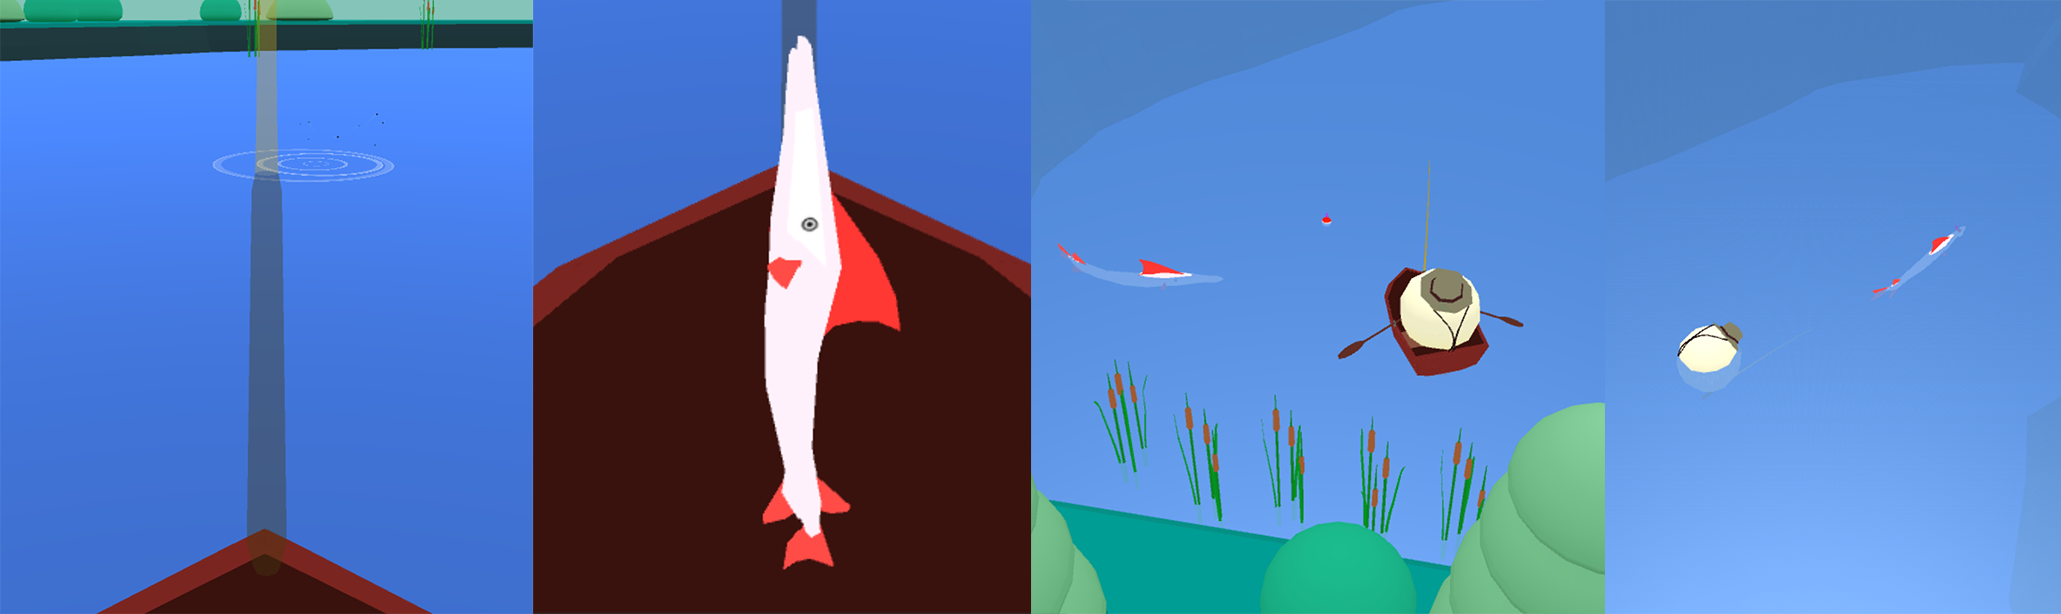
\includegraphics[width = \paperwidth]{Golf/Fishing}}
    \caption{Left: First-Person Fishing. Right: Golfing as a Fish}
    \label{Fishing}
  \end{figure}
\end{center}
\subsubsection{Domino Golf}
Domino is a game of its own, but the domino pieces themselves can also be used to create a sequence of aligned pieces that when toppled creates a satisfying domino effect, hence the name of the effect. For this level I wanted to capture this feeling. I quickly realised, 1) that the game engine on its own could not quiet capture this satisfactory collision when ivory meets ivory, and 2) the arduous work of aligning massive amounts of domino pieces. Thus, the first two challenges were identified. In addition to the first challenge, I also wanted to incorporate scale as an element in the collision feel: Small pieces colliding with other small pieces should progress fast and the opposite for large pieces, therefore I tied the overall timescale with the most current collision, so that, the smaller the piece the faster time progressed. This gave the desired illusion but proved ill-fitting when other elements undesirably got drawn into this time altering. Instead, a combination of increasing or decreasing the piece's velocity and the gravity acted upon it according to the piece's scale, was implemented. For the second challenge I needed a tool that could assist in setting up the domino pieces in a line, but not a straight line. I implemented a method that could place domino pieces according to an unlimited amount of segments containing a Bezier curve. Further, I made the line visible in a simplified version outside of play mode, to better determine the path. Finally, I made an accompanying two-dimensional graph for determining scale in the course of the line.

Next, was the problem of what to control. I determined that it should be a domino piece, and this proved to be difficult because of the shape. It is quiet difficult to build up speed when the dimensions of the projectile is highly unbalanced. The long rectangular shape of a domino piece, simply, is not made for speed. This meant, that the first iteration of the domino controller felt very much like a fish out of water, not meant to travel across the ground. At this point, I was trying to determine whether or not this was what I wanted. After all, a golf field is not a domino piece's natural habitat. I decided to iterate nonetheless: Instead of just forcing the piece across the level, I decided to, when the player touches the screen, alter the posture of the piece to a standing one, and then when the player releases, boost the piece forward in a handspring-manner (flick flack). This felt extremely satisfactory and how I felt a domino piece would traverse a golf field.
\begin{center}
  \begin{figure}[!htb]
    \noindent\makebox[\textwidth]{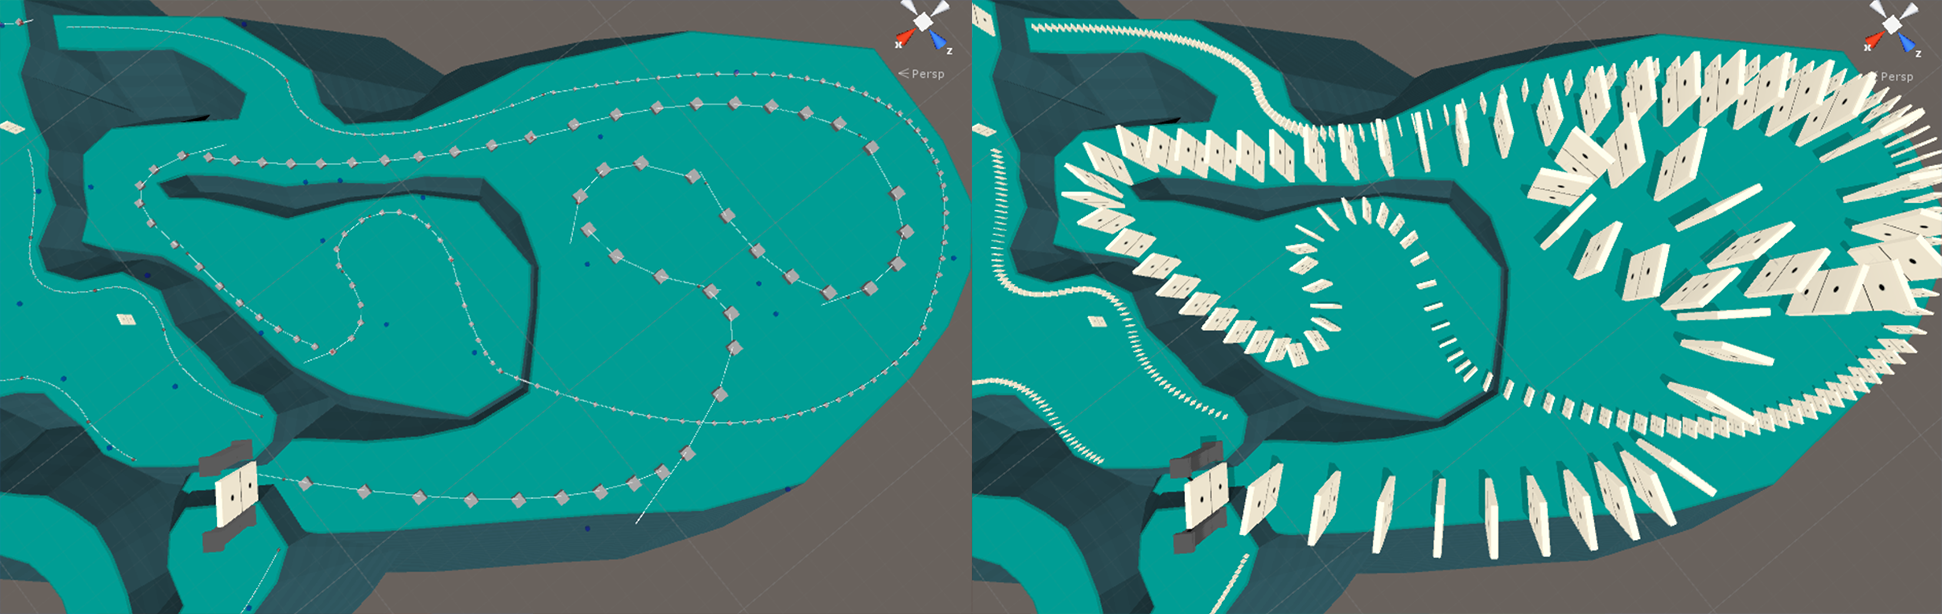
\includegraphics[width = \paperwidth]{Golf/Domino}}
    \caption{Left: Domino Pieces Visualised outside of Play Mode. Right: In Play Mode}
    \label{Domino}
  \end{figure}
\end{center}
\subsubsection{Sonic Golf}


\subsection{Summary}


\section{Reflection}
The following sections will contain my most noteworthy reflections during my internship at Triband.
\subsection{Agility}
Triband work fast. \citeA{buxton} describes sketching as being quick to make, can be made when needed, the cost of it is not prohibiting, disposable once its use is depleted and it is plentiful in quantity. These are all characteristics that can describe the current levels in Golf All the Things. The creation of a level starts with a wacky idea, it is written on a post-it and pinned to the "New" board. The post-its are only descriptive in a minimal sense and the work only really begins inside the game engine. The perhaps most used sketching application is in the medium of pen and paper, however, I would argue that because of a high expertise in the toolset for creating games, Triband are using these tools as a sketching method. As of writing, Golf All the Things has over 200 levels, whereas about 20\% is expected to make it to the final game. I really appreciate this approach to game design since it requires the designer to really pinpoint what the interesting thing about his/her idea is, and after it is implemented, move on. Then, as a second phase the game designers can go through the sketches and decide which ones to develop further. Of course, this method requires a high amount of practicing and cannot be adopted by novices, but in my opinion it is a great method both for the development of games but also as an initial exploration of different game ideas. One that is definitely worth the effort of learning tools such as rough 3D modelling, illustration, game engines and programming.
\subsection{Programming as a Design Tool}
Being in a small studio, no one really had time to assist in the creation of prototypes other than advice. This meant that to actually create a prototype I had to program. I have taken programming courses outside of my study program, so I had some experience before my internship started, but had I not had this, I would not have been able to design any levels. In the near future, after graduating, I expect this to be relevant since I am not expecting to get hired in a position where I am able to assign design tasks without at least being able to complete these tasks myself. While I might be able to acquire such a position eventually, I am expecting my programming skills to be of importance on the other side of graduating.

Another argument for programming as a design tool is the inspiration that can come from bugs. When I program I rarely get the desired solution in the first run. This means that situations arise that I would not have thought of myself, and this can, in turn, lead to a more interesting solution or at least a higher degree of certainty in your desired solution. A concrete example of this is the shooter control for the domino piece in my domino level. My first iteration of this was a shooter control that applied the right balance of force and rotation force for the piece to somewhat move in the player's desired direction, but it felt clunky. This lead me to the trail of thought of, yes, perhaps a domino would be like a fish out of water as soon as it is taken out of a usual domino context, which in turn lead me to think, no, the domino should not control like a fish, but instead utilise its abnormal shape in an optimal way. And thus, the final iteration was made with me feeling a higher amount of affirmation than I would have otherwise felt, had I come up with the final iteration immediately.

A final justification for designers learning to program: You can create your own tools. When I was creating the domino levels I needed a tool for aligning pieces in the game world. With programming, I could. This example did end up being probably the most advanced thing I have programmed, testifying that some experience is required to use programming in this way.


\newpage
\bibliography{bib}

\end{document}
